\chapter{Calibration de la mesure de courant}

La carte électronique UCM Nano est capable de réaliser des mesures de tension, courant, résistance, température, fréquence, rapport cyclique et l'état d'un signal logique. 

\section{Séquences de test sur TestStand}

Pour calibrer la carte électronique il faut calculer le gain et l'offset à partir des mesures avec un multimètre (données calibrées) et des mesures directes de la carte UCM Nano (données pas calibrées).

Dans le développement de notre plan de test, nous avons défini des scénario de test ; des étapes de test ; des pas de test et des fonctions. Les fonction sont des briques de base utilisés dans les pas de test, ceux-ci font des pas basique que seront utilisés par des étapes de tests, chaque étape de test est composée par une séquence de pas basiques qui font une tâche plus complexe. Dans chaque scénario de test, ce sont réalisés des tests complètes pour différents types de dispositif sous test et/ou différents configurations du dispositif sous test.

Nous avons deux scénarios de test : Standard 0 et Standard 3. Quelles sorties et ses respectives valeurs de courant pour chaque standard sont affichés sur le tableau \ref{tab:calibration-selon-variantes}.


\begin{table}[H]
\centering
\caption{Calibration selon les variantes : standard 0 et standard 3.}
\label{tab:calibration-selon-variantes}
\begin{tabular}{|c|c|c|c|c|}
\hline
 \multirow{2}{4em}{\textbf{ Sortie }} & \multicolumn{2}{|c|}{ \textbf{ Standard 0 }} & \multicolumn{2}{|c|}{ \textbf{ Standard 3 }} \\
\cline{2-5}
 & \textbf{ Type } & \textbf{ I$_{max}$ (A) } & \textbf{ Type } & \textbf{ I$_{max}$ (A) }  \\
 \hline
 & & & & \\
\hline
 \textbf{LSD-01} & LSO10a & 2 & & \\
\hline
 \textbf{LSD-09} & LSO6a & 3 & & \\
\hline
 \textbf{LSD-10} & LSO6a & 3 & & \\
\hline
 \textbf{LSD-11} & LSO6a & 3 & & \\
\hline
 \textbf{LSD-12} & LSO13a & 7 & & \\
\hline
 & & & & \\
\hline
 \textbf{HSD-01} & HSO1a & 0,22 & & \\
\hline
 \textbf{HSD-02} & HSO16a & 2,5 & HSO1b & 0,22 \\
\hline
 \textbf{HSD-03} & HSO33a & 3 & & \\
\hline
 \textbf{HSD-04} & HSO27a & 3,5 & & \\
\hline
 \textbf{HSD-05} & HSO33a & 3 & & \\
\hline
 \textbf{HSD-07} & HSO34a & 4 & & \\
\hline
 \textbf{HSD-08} & HSO12a & 6,4 & HSO12a & 6,4 \\
\hline
 \textbf{HSD-09} & HSO15a & 4,5 & HSO15a & 4,5 \\
\hline
 \textbf{HSD-10} & HSO25a & 0,5 & & \\
\hline
 \textbf{HSD-11} & HSO8a & 2,5 & & \\
\hline
\end{tabular}
\end{table}

Chaque type de sortie est déterminé par certaines caractéristiques que la sortie doit avoir. Si elle a un pull-down (LSO - Low Side Output) ou un pull-up (HSO - High Side Output) ; à quelle valeur de courant maximale elle peut fournir et quel est la classe de la charge qu'elle doit piloter :

\begin{itemize}
\item a -> une self (bobine),
\item b -> une diode LED,
\item c -> un relai,
\item d -> une résistance.
\end{itemize} 

Nous avons séparé les séquences de test sur TestStand dans trois catégories : étapes de test, pas de test e fonction de test. 


\begin{itemize}
\item Les étapes de test : 
\subitem Output calibration, 
\subitem Measure of current ;

\item Les pas de test : 
\subitem Write to the UCM, 
\subitem Read from the UCM, 
\subitem Manage CAN response, 
\subitem Connect load, 
\subitem Connect UCM output, 
\subitem Connect supply ;

\item Les fonctions de test : 
\subitem Convert CAN response to number, 
\subitem Manage CAN error, Write to RAM memory, 
\subitem Write to FLASH memory, 
\subitem Read from the digital multimeter, 
\subitem Switch initialization, 
\subitem Connect/disconnect switch, 
\subitem Close switch.
\end{itemize}
 



\section{Connection de la sortie et des charges}

Nous connectons les sorties de la carte UCM Nano et les charges par des interrupteurs. La banque d'interrupteurs utilisé est la \textit{5A Power EMR MUX Module}, code du modèle chez \emph{Pikering} : 40-651-014. Pour piloter cette carte, et d'autres modules, nous avons utilisé un châssis avec 18 \textit{slots}.


\begin{figure}[H]
    \centering
    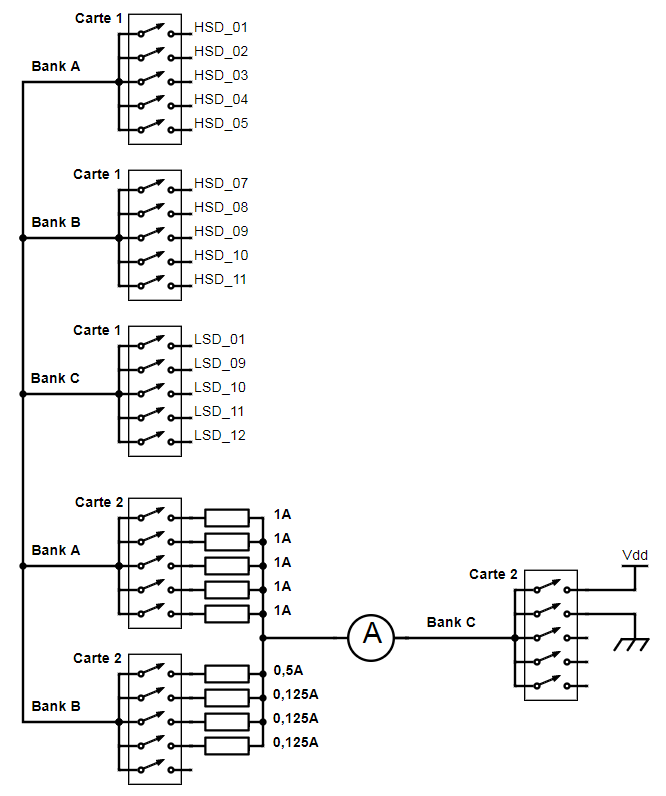
\includegraphics[width=0.80\textwidth]{images/switches-carte1-2}
    \caption{Connection des sorties de l'UCM Nano et des charges avec les banques d'interrupteurs.}
    \label{fig:switches-carte1-2}
\end{figure}


\section{Activation des sorties de l'UCM Nano}


\section{Mesure du courant}

\subsection{Mesure de courant avec le multimètre}



\subsection{Mesure de courant avec la carte}



\section{Calcule du gain et de l'\textit{offset}}





\section{Écriture dans la mémoire}



%\section{Vérification de la calibration}